
\begin{figure}[htbp]
    \centering
    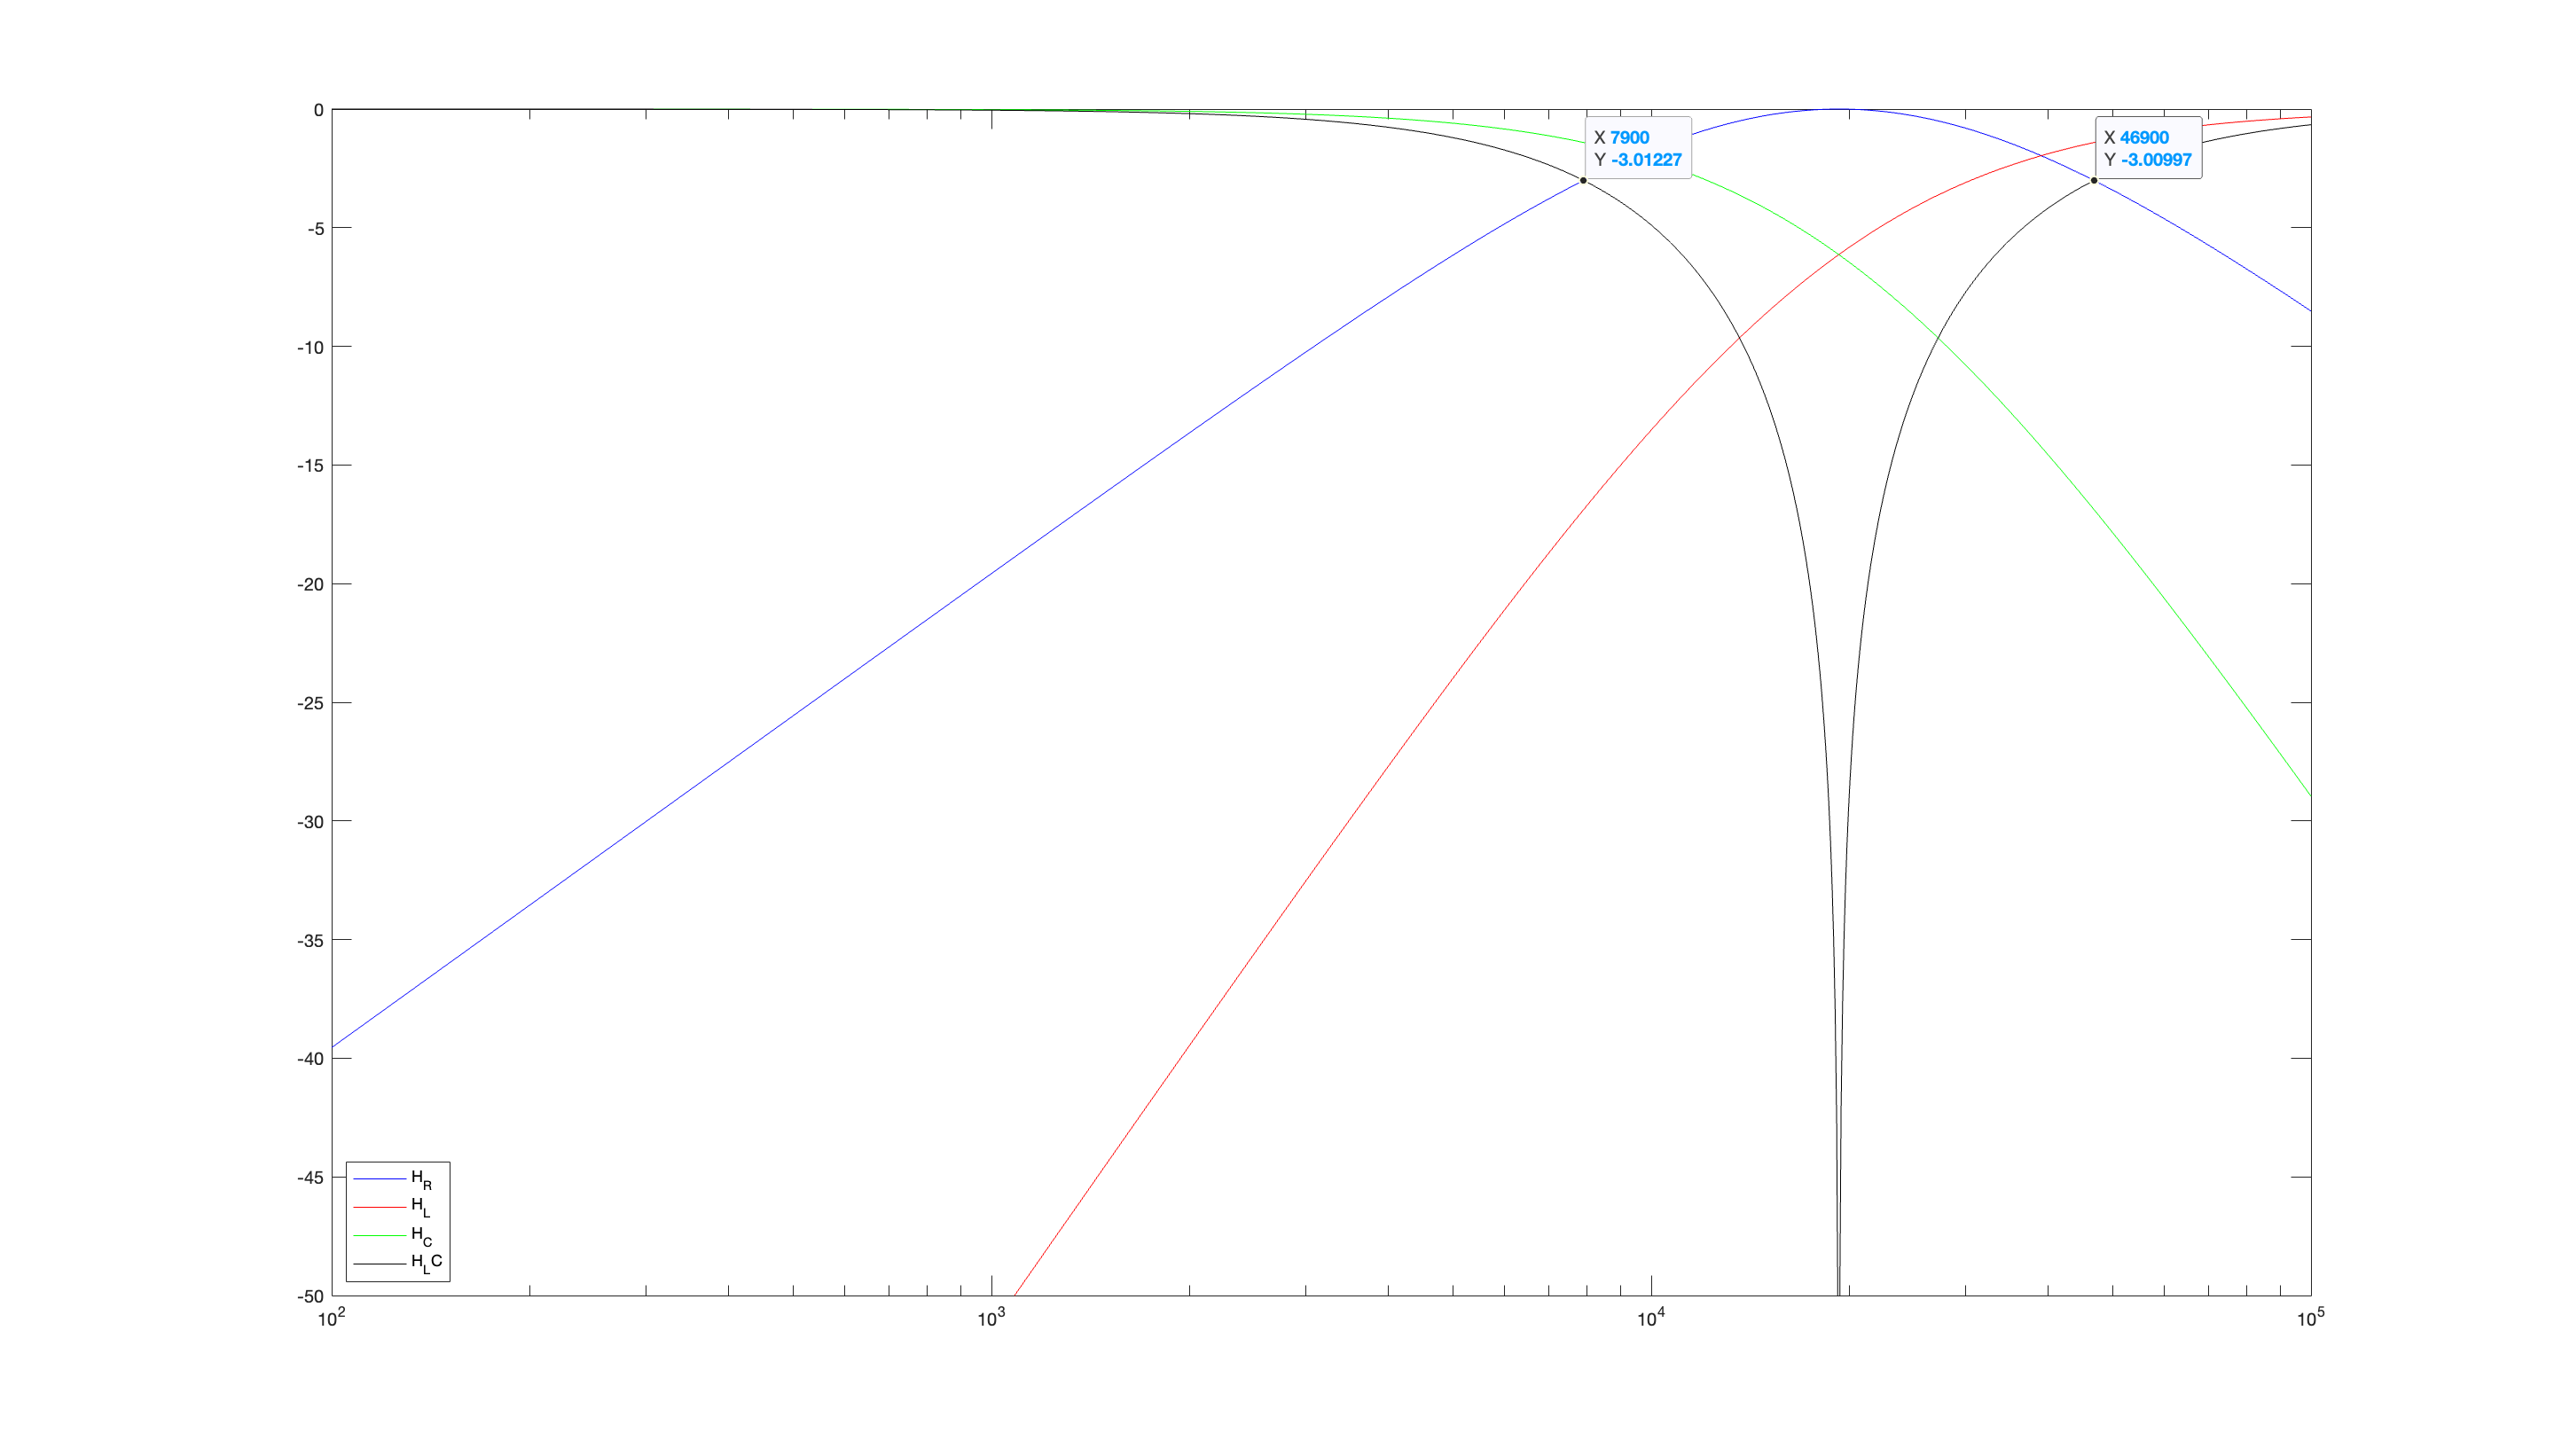
\includegraphics[width=\textwidth]{images/prelab/parallel_RLC_series_plot.png}
    \caption{RLC Series Voltages taken over different components}
    \label{fig:prelab}
\end{figure}

From the plot, we find that the corner frequencies are given as
\begin{equation}
    \omega _1 = 7.9E3 \text{ rad/s} \text{ and } \omega _2 = 4.69E4 \text{ rad/s}
\end{equation}


We also find that the bandwidth is, in the series RLC circuit:

\begin{center}
    {\bf Calculated}: $3.9E4$
    \\
    {\bf Plotted}: $3.9E4$
\end{center}

The quality factor is calculated to be(by knowing that $Q = \frac{X_0}{R} = \frac{\sqrt{\frac{L}{C}}}{R}$)

\begin{center}
    \(Q=0.49346\)
\end{center}

We find that the voltage taken over the resistor makes the circuit act as a {\bf bandpass} filter, the voltage taken over the
inductor makes the circuit act as a {\bf high-pass} filter,
the voltage taken over the capacitor makes the circuit act as a {\bf low-pass} filter, and the voltage taken over the inductor and the capacitor makes the circuit act as a {\bf band-stop} filter.
The bode magnitude of the RLC series circuit plot and the MATLAB code used to obtain the corner frequencies and create the plot is given below:
\begin{verbatim}
R = 390; % in ohm
C = 270E-9; % in F
L = 10E-3; % in H

w = 100:100:100E3;
jw = 1i*w;

% Voltage over the resistor
H_r = (jw .* (R .* C)) ./ ((jw.^2 .* L .* C) + (jw .* R .* C) + 1);

semilogx(w, 20 * log10(abs(H_r)), "blue");

hold on

% Voltage over the inductor
H_l = (jw.^2 .* L .* C) ./ ((jw.^2 .* L .* C) + (jw .* R .* C) + 1);
semilogx(w, 20 * log10(abs(H_l)), "red");

% Voltage over the capacitor
H_c = 1./((jw.^2 .* L .* C) + (jw .* R .* C) + 1);
semilogx(w, 20 * log10(abs(H_c)), "green");

% Voltage over the inductor and the capacitor
H_lc = ((jw.^2 .* L .* C) + 1) ./ ((jw.^2 .* L .* C) + jw .* R .*C + 1);
semilogx(w, 20 * log10(abs(H_lc)), "black");
ylim([-50, 0]);

legend("H_R", "H_L", "H_C", "H_LC", "Location", "southwest")

% Calculated bandwidth and quality factor:
B_calculated = R/L;
w_0 = 1/sqrt(L*C);
X_0 = sqrt(L/C);
Q_s = X_0/R;

w_2 = 4.69E4;
w_1 = 7.9E3;

B_plot = w_2 - w_1;

disp("Plot Bandwidth: " + (w_2 - w_1));

disp("Calculated Quality Factor: " + Q_s);
disp("Calculated Bandwidth: " + B_calculated);
\end{verbatim}

\subsection{Execution and Experiment Data}
A series RLC resonant circuit was implemented with $R=390\Omega, C=270nF, L=10mH$. The circuit was driven by a function generator in log sweep mode at 5$V_{pp}$ without an offset, with the frequency being varied every 500ms from 100Hz to 100kHz.

For $V_R, V_C, V_L, V_{CL}$ the following hardcopies are shown:

\begin{figure}[H]
    \centering
    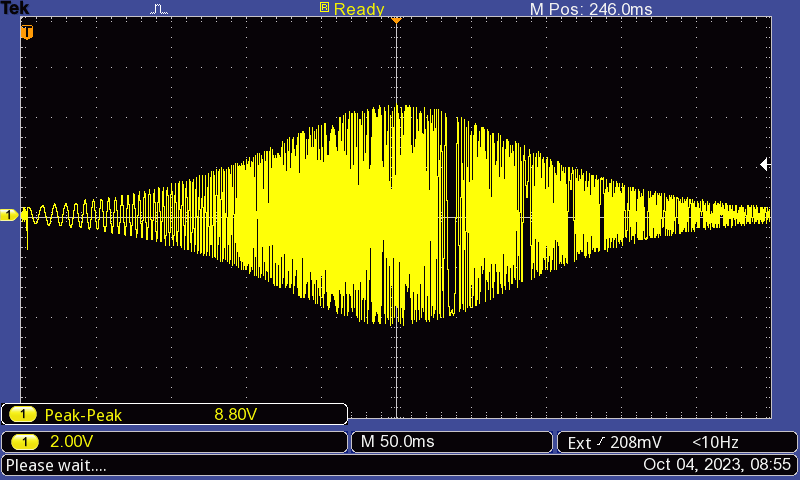
\includegraphics[width=0.5\textwidth]{images/prelab/V_R.png}
    \caption{Voltage over the resistor showing band-pass behavior}
    \label{fig:prelab_Vr}
\end{figure}

\begin{figure}[H]
    \centering
    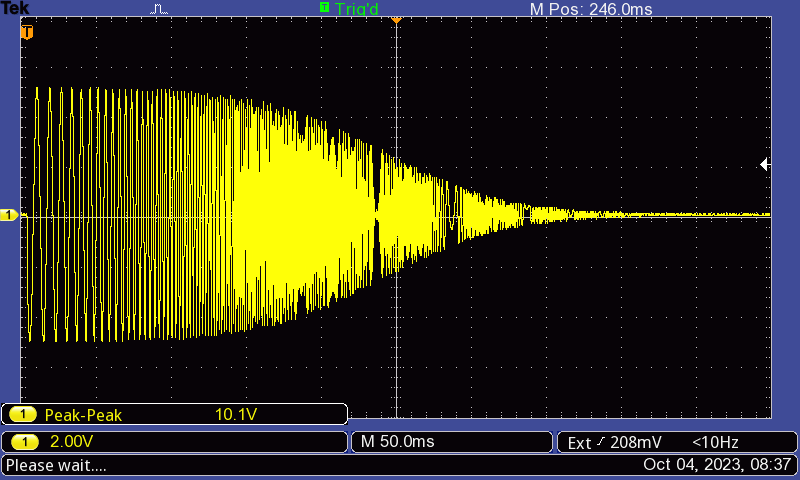
\includegraphics[width=0.5\textwidth]{images/prelab/V_C.png}
    \caption{Voltage over the capacitor showing low-pass behavior}
    \label{fig:prelab_Vc}
\end{figure}

\begin{figure}[H]
    \centering
    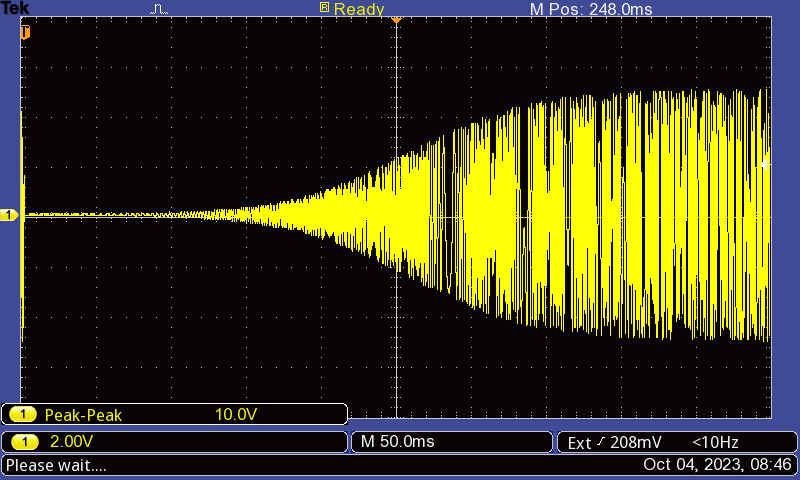
\includegraphics[width=0.5\textwidth]{images/prelab/V_L.png}
    \caption{Voltage over the inductor showing high-pass behavior}
    \label{fig:prelab_Vl}
\end{figure}

\begin{figure}[H]
    \centering
    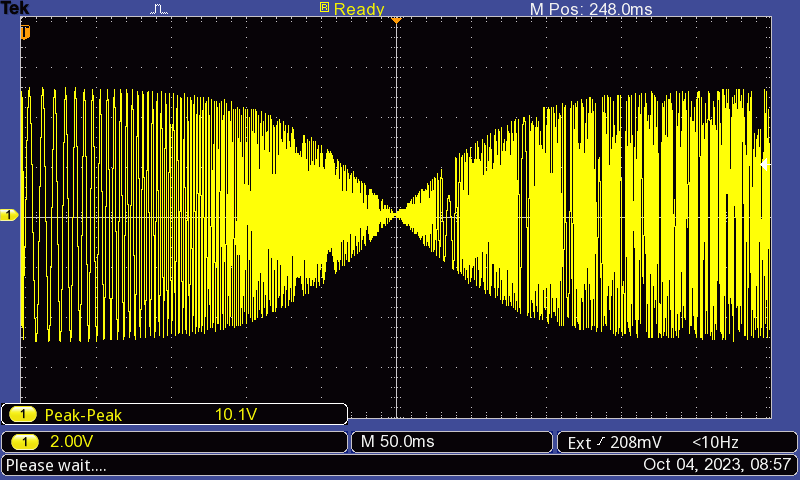
\includegraphics[width=0.5\textwidth]{images/prelab/V_CL.png}
    \caption{Voltage over the capacitor and inductor showing band-stop behavior}
    \label{fig:prelab_Vcl}
\end{figure}

For the next part, the circuit is configured to be band-pass once more. It was observed that the Lissajou figure could be used to determine whether the frequency provided is above or below the resonant frequency. If the Lissajou figure is linear, then the frequency is the resonant frequency. It was found that the frequency at which the Lissajou figure turns linear is around $3100\text{Hz}$.

\begin{figure}[H]
    \centering
    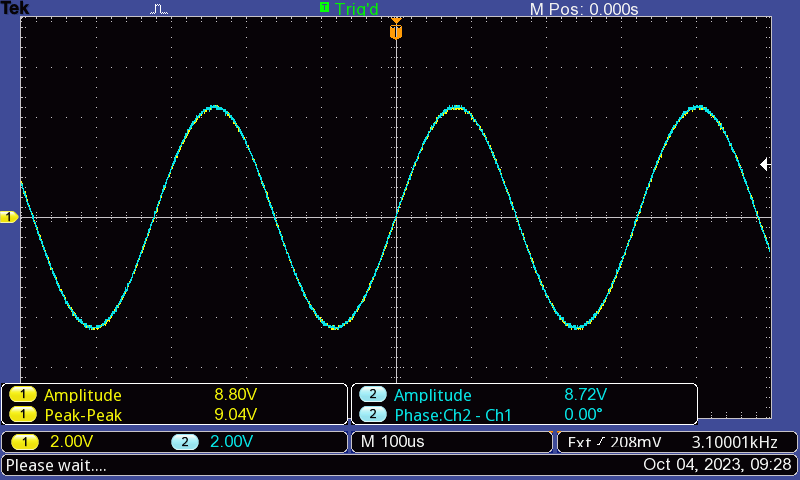
\includegraphics[width=0.75\textwidth]{images/prelab/phase_V_R.png}
    \caption{The phase difference between the input and the output voltage over the resistor is shown to be 0deg at the resonant frequency}
\end{figure}

The corner-frequencies were found to be 1290Hz and 7640Hz respectively,
very close to nominal frequencies when compared:
$f_1 \times 2\pi = 8105\text{rad/s}$ and $f_2 \times 2\pi = 48000\text{rad/s}$.